\chapter{Text Extraction and Summarization}

\indent\indent The first part of this chapter gives a brief description of text extraction method used in our project and its internal working. The second part explains the text summarization algorithm.  
\section{Text extraction}
Optical Character Recognition (OCR) is the process of
converting any form of text or text-containing documents such as handwritten text, printed or scanned text images, into an editable digital format for deeper and further processing. \cite{hamad2016detailed}
Tesseract is an open source text recognition (OCR) Engine, available under the Apache 2.0 license. It can be used directly, or (for programmers) using an API to extract printed text from images. It can be used with the existing layout analysis to recognize text within a large document, or it can be used in conjunction with an external text detector to recognize text from an image of a single text line.\\
Tesseract 3.x was dependant on the multi-stage process:
\begin{enumerate}
    \item Word finding
    \item Line finding
    \item Character classification
\end{enumerate}

Word finding is done by organizing text lines into blobs, and the lines and regions are analyzed for fixed pitch or proportional text. Text lines are broken into words differently according to the kind of character spacing. Recognition then proceeds as a two-pass process. In the first pass, an attempt is made to recognize each word. Each word that is satisfactory is passed to an adaptive classifier as training data. The adaptive classifier then recognizes the text accurately.

Modernization of the Tesseract tool was an effort on code cleaning and adding a new LSTM (Long Short Term Memory networks) model. The input image is processed in boxes (rectangle) line by line feeding into the LSTM model and giving output. 

% \ref{fig:extract} 
\begin{figure}[H]
\centering
	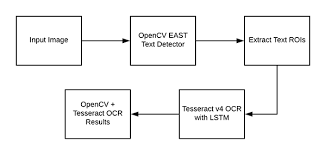
\includegraphics[scale=1]{Figures/extract.png}	
	\caption{Text extraction}
	\label{fig:extract}
\end{figure}

\section{Summarization}
Summarization \cite{reddy2012efficient} is the process of compressing the original document into a short summary by extracting the most important information from the document. The summary of the document can be helpful to the user to get the main theme of the document in a short span of time. The flow of information in a given document is not uniform, which means that some parts are more important than others. The important task in summarization lies in distinguishing the more informative parts of a document from the less ones.\\
Extractive vs. Abstractive summarization: 
\begin{enumerate}
    \item An extractive summarization method is the process of selecting most important sentences from the original document
    \item An abstractive summarization method produces a short summary by rephrasing the sentences that convey the same information. It involves natural language processing.\\ 
\end{enumerate}
Extractive summaries \cite{madhuri2019extractive} can be formulated by extracting the text segments (sentences or paragraphs) from the text based on the term frequency and sentence similarity. \\
There are several scenarios where automatic construction of summaries is useful. Other examples include automatic construction of summaries of news articles or email messages for sending them to mobile devices as SMS; summarization of information for government officials, business persons, researches, etc., and summarization of web pages to be shown on the screen of a mobile device, among many others. The Extraction based summarization methods will extracts the most important sentences from the given document. The main challenge of document summarization is to decide which sentences from the input document should be included in a summary. It first, assigns a score to each sentence and then gives ranks to the sentences according to their scores. The sentence with highest score will get the top rank. The score for a sentence is calculated by using statistical features including sentence position, cue words, term frequency, document frequency, topic signature, etc. \\
Text Summarization is the art of abstracting key content from information sources. Text summarization is one of the many applications of natural language processing and is becoming more popular for information condensation. Natural Language Processing played an important role developing the summary from a large extract. Concepts such as stemming and lemmatization was crucial in the development of the summary. Stemming ensures that all similar words are normalized while lemmatization ensures that infected words were mapped to their healthy dictionary forms. The summarization was done on the basis of eliminating less important sentences from the extract and concurrently keeping the more important ones. The usefulness of a sentence was judged based on the frequency of relevant words in it. The Natural Language Toolkit (NLTK) is used in our project for text summarization.\\
% \ref{fig:summarizer} 
\begin{figure}[H]
\centering
	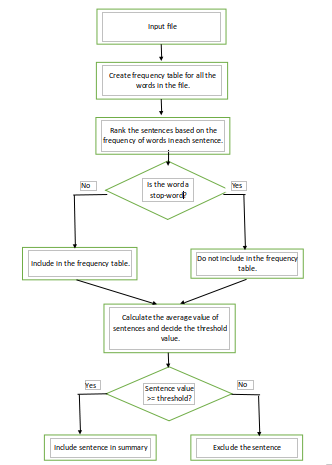
\includegraphics[scale=1]{Figures/summarizer.png}	
	\caption{Summarization Flow}
	\label{fig:summarizer}
\end{figure}


\vspace{0.75cm}
In summary, text extraction is a process of generating text from electronic documents that have associated text. The tesseract module of python uses OCR to extract text from images. Text summarization is a method of removing redundant information from text by using frequency tables. Natural language toolkit is used for achieving this.
  